% siminos/atlas/flotsam.tex    master file: main.tex
% $Author$ $Date$

\section{Flotsam}
\label{s:flotsam}

\noindent
{\bf [2012-03-12 Predrag]}
\\
How to use this section? When you remove cogent text from the article
proper - clip  it and paste it into here, for possible reuse later.

\subsection{Introduction}
\label{s:introFlot}

This paper has two ideas:
\begin{enumerate}
  \item slice locally
  \item chart globally
\end{enumerate}

    \begin{itemize}
      \item closest point on a group orbit
      \item variation $\to$ \slice\ hyperplane
    \end{itemize}

    in order to motivate the need for continuous symmetry reduction , explain
    what it is, and how with it the geometry of \statesp\ dynamics is revealed;

We review  ??? flows, their visualization, and their symmetries in
\refsect{s:review}. The {\mslices}  is described in \refsect{s:slice},
and the computation of invariant solutions and their stability
eigenvalues and eigenvectors in \refsects {sect:TimeOrb}{s:algorithm}.
The main advances reported in this paper are the symmetry \reducedsp\
visualization and [...], (\refsect{s:rpos}). Outstanding challenges are
discussed in \refsect{s:concl}.

% \subsection{Pipe flows}
% \label{s:reviewFlot}
% former siminos/atlas/review.tex    master file: main.tex

On perils of thinking linearly: bases such as Fourier modes are
perfectly natural for problems such a bifurcation of a steady state, and
other weak perturbations. They are absolutely unnatural for strongly
nonlinear problems, with many Fourier modes of comparable magnitude and
strongly entangled.

        There is always tension between mathematics - linear problem eigenmodes
        (Fourier for translations and rotations) and physics - the fact that
        nonlinear dynamics states are far away from such axes, as they
        always involve a number of such linear modes strongly entangled.

\subsubsection{Experimentalist description: a video 1D to 3D arrays of pixels}
\subsubsection{Theorist description: $\infty$-\dmn\ \statesp}

\subsection{Poincar\'e sections}
\label{s:PoincSecFlot}

%%%%%%%%%%%%%%%%%%%%%%%%%%%%%%%%%%%%%%%%%%%%%%%%%%%%%%%%%%%%%%%%%%%%%
\begin{figure}
   \centering
(a)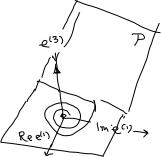
\includegraphics[width=0.20\textwidth]{A29PoincBad}
(b)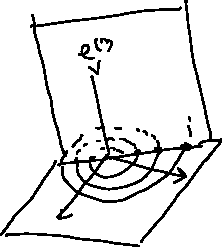
\includegraphics[width=0.20\textwidth]{A29PoincGood}
   \caption{\label{fig:A29PoincBad}
A Poincar\'e section should capture important features of the local flow.
    (a)
A section through a \template\ off the invariant set is bad, as it misses
dynamics around a nearby \eqv.
    (b)
If an \eqv\ is chosen as a \template, the section is good - it captures
all local dynamics.
}
\end{figure}
%%%%%%%%%%%%%%%%%%%%%%%%%%%%%%%%%%%%%%%%%%%%%%%%%%%%%%%%%%%%%%%%%%%%%

%%%%%%%%%%%%%%%%%%%%%%%%%%%%%%%%%%%%%%%%%%%%%%%%%%%%%%%%%%%%%%%%%%%%%
\begin{figure}
   \centering
   %\includegraphics[width=0.45
\begin{minipage}[b]{0.19\textwidth} %{0.39\textwidth}
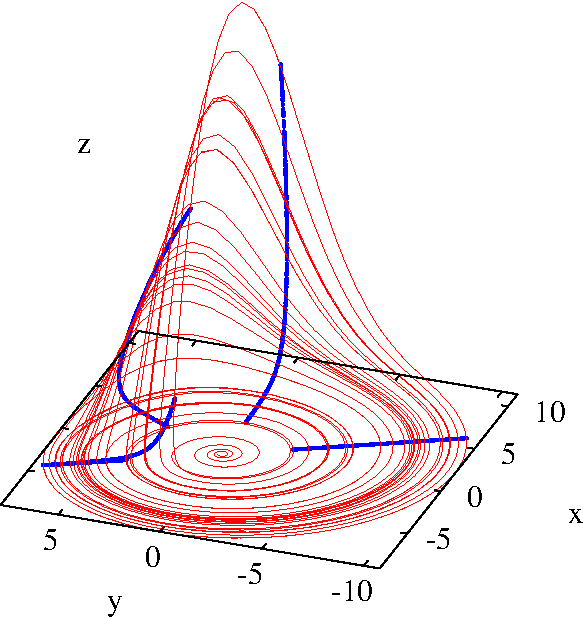
\includegraphics[width=1.15\textwidth,origin=c]
            {Rossler_PsectionB}
\\
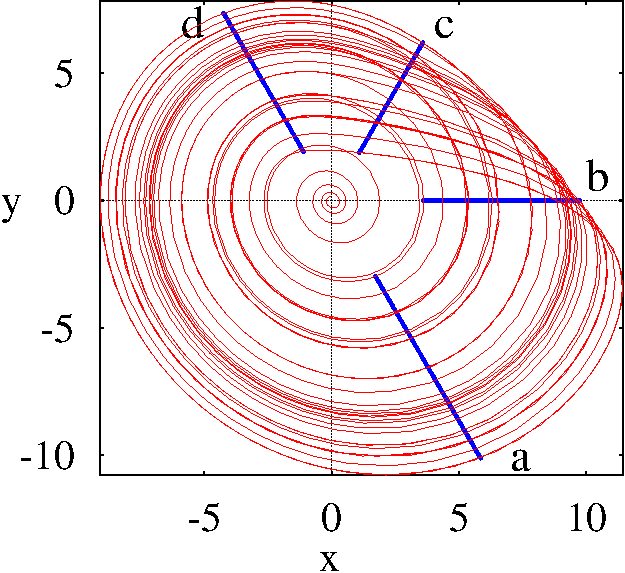
\includegraphics[width=0.80\textwidth,origin=c]
            {Rossler_PsectionA}
  \end{minipage}~~~~~%
  \begin{minipage}[b]{0.25\textwidth} %{0.50\textwidth}
    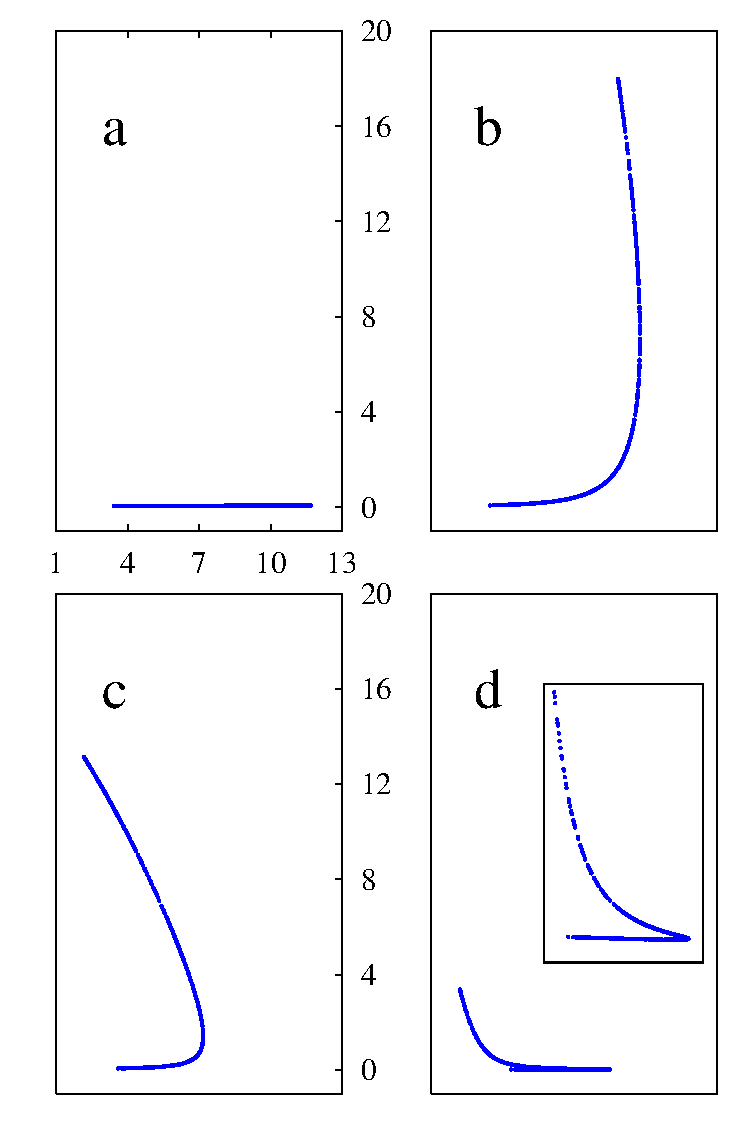
\includegraphics[width=1.00\textwidth]
            {Rossler_PsectionC}
  \end{minipage}
   \caption{\label{f:RosslSect}
      (Right) a sequence of Poincar\'e sections of
      the R\"ossler strange attractor,
      defined by planes through the $z$~axis, oriented at angles
      (a) $-60^o$
      (b) $0^o$,
      (c) $60^o$,
      (d) $120^o$,
      in the $x$-$y$~plane.
      (Left) side and $x$-$y$~plane view of a typical trajectory  with
      Poincar\'e sections superimposed.
      (R. Pa\v skauskas)
            }
\end{figure}
%%%%%%%%%%%%%%%%%%%%%%%%%%%%%%%%%%%%%%%%%%%%%%%%%%%%%%%%%%%%%%%%%%%%%

%%%%%%%%%%%%%%%%%%%%%%%%%%%%%%%%%%%%%%%%%%%%%%%%%%%%%%%%%%%%%%%%%%%%%
% \label{fig:RoessNearEq1}
\begin{figure}
(a)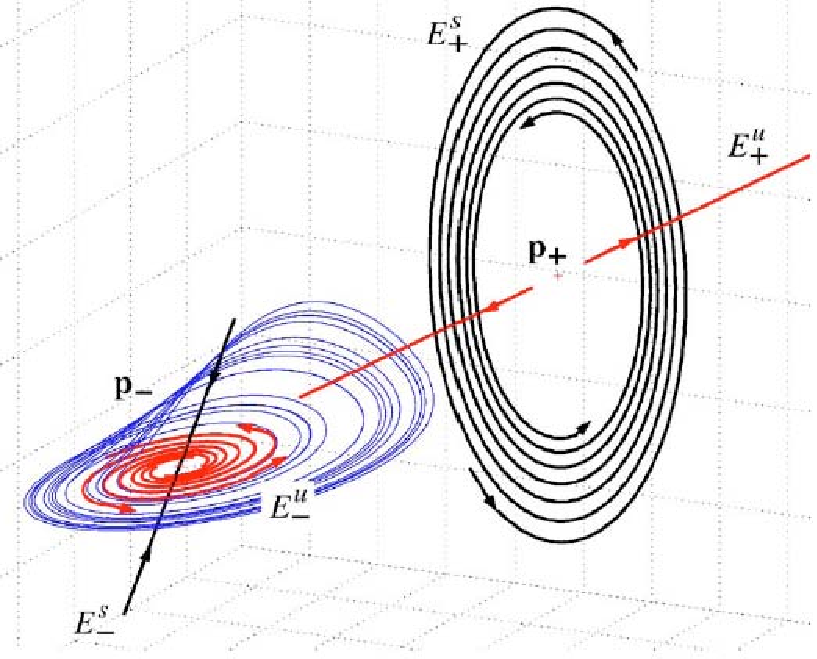
\includegraphics[width=0.3\textwidth]{AmLeAg06Im1}
(b)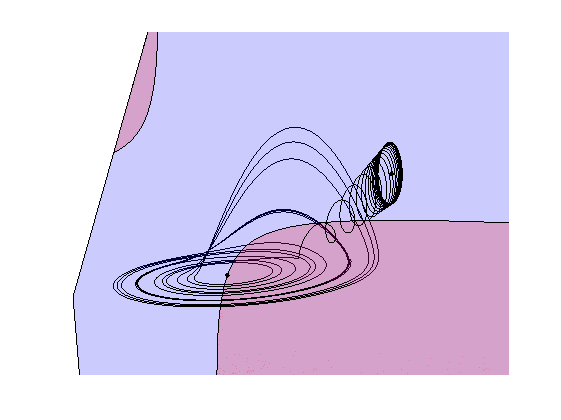
\includegraphics[width=0.30\textwidth,clip=true]{RoessNearEq}
    \caption{[From \refref{AmLeAg06}]
(a)
R\"ossler \eqva\ and their invariant manifolds. The stable manifold of
the inner {\eqv} $\ssp_{-}$  is 1-dimensional and the unstable one is a
spiral-out focus. For the outer {\eqv} $\ssp_{+}$  the stable manifold is
a spiral-in focus (basin boundary for initial conditions that either fall
into the chaotic attractor, or escape to infinity) and the unstable
manifold is 1-dimensional.
(b)
  A R\"ossler flow Poincar\'e section $\PoincS_{-}$ through the inner
  {\eqv} $\ssp_{-}$ and its stable eigenvector.
    }
\label{fig:AmLeAg06Im1}
\end{figure}
%%%%%%%%%%%%%%%%%%%%%%%%%%%%%%%%%%%%%%%%%%%%%%%%%%%%%%%%%%%%%%%%%%%%%

%%%%%%%%%%%%%%%%%%%%%%%%%%%%%%%%%%%%%%%%%%%%%%%%%%%%%%%%%%%%%%%%%%%%%
% \label{fig:RoessBothEq1}
\begin{figure}%[H]
\begin{center}
(a)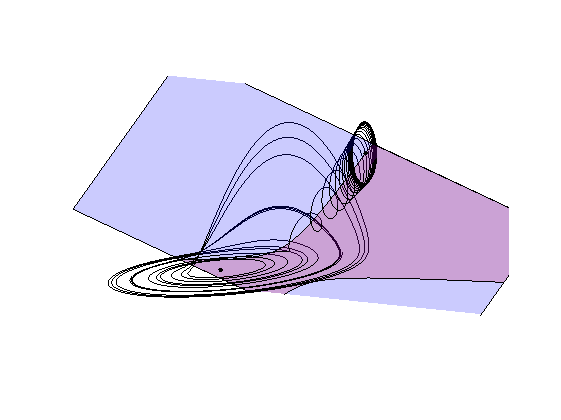
\includegraphics[width=0.30\textwidth,clip=true]{RoessFarEq}
(b) 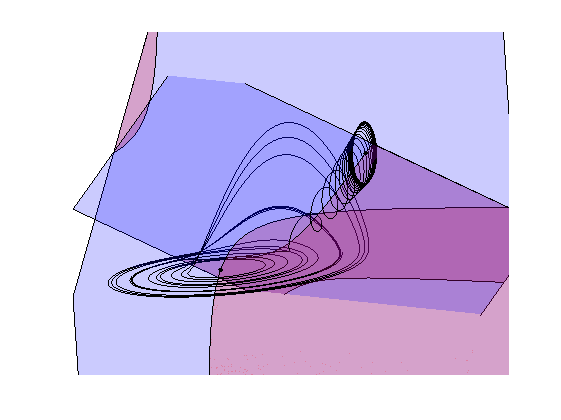
\includegraphics[width=0.30\textwidth,clip=true]{RoessBothEq}
\end{center}
  \caption[R\"ossler section, outer {\eqv}]{
(a) A Poincar\'e section for R\"ossler flow through the outer {\eqv}
$\ssp_{+}$  and its unstable eigenvector.
(b)
  A two-section atlas for R\"ossler flow, with the local sections of
  \reffigs{fig:RoessNearEq}{fig:RoessFarEq} oriented and combined so that
  the ridge (intersection of the two sections, indicated by the brown
  line in individual sections) lies  approximately midway between the
  \template s.
  } \label{fig:RoessFarEq1}
\end{figure}
%%%%%%%%%%%%%%%%%%%%%%%%%%%%%%%%%%%%%%%%%%%%%%%%%%%%%%%%%%%%%%%%%%%%%

%%%%%%%%%%%%%%%%%%%%%%%%%%%%%%%%%%%%%%%%%%%%%%%%%%%%%%%%%%%%%%%%%%%%%
% \label{fig:RoessSct2} \label{fig:RoessSctAtlas}
\begin{figure}%[H]
\begin{center}
(a)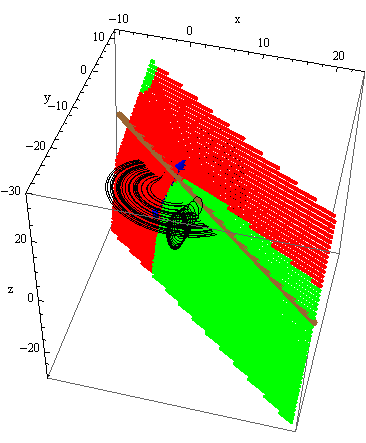
\includegraphics[width=0.30\textwidth,clip=true]{RoessSct1}
(b) 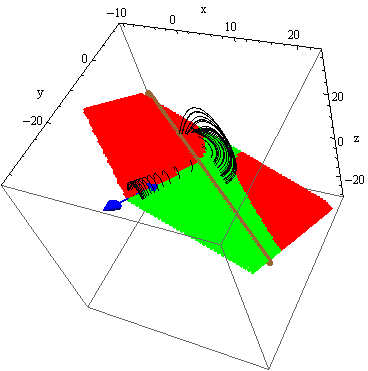
\includegraphics[width=0.30\textwidth,clip=true]{RoessSct2}
(c) 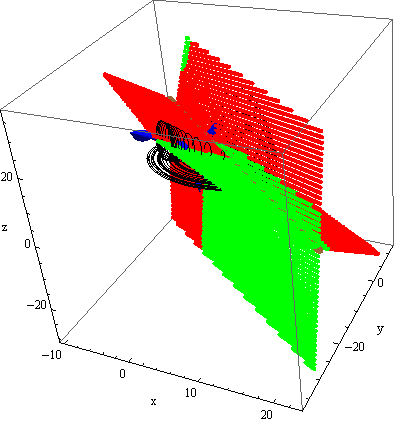
\includegraphics[width=0.30\textwidth,clip=true]{RoessSctAtlas}
\end{center}
  \caption{\label{fig:RoessSct1}
(a) A R\"ossler flow Poincar\'e section $\PoincS_{-}$ through the inner
  {\eqv} $\ssp_{-}$ and its stable eigenvector.
(b)
  A Poincar\'e section for R\"ossler flow
      through the
      outer
  {\eqv} $\ssp_{+}$  and its unstable eigenvector
(c)
  A two-section atlas for R\"ossler flow, with the local sections of
  \reffigs{fig:RoessSct1}{fig:RoessSct2} oriented and combined so that
  the ridge (intersection of the two sections, indicated by the brown
  line in individual sections) lies  approximately midway between the
  \template s.
}
\end{figure}
%%%%%%%%%%%%%%%%%%%%%%%%%%%%%%%%%%%%%%%%%%%%%%%%%%%%%%%%%%%%%%%%%%%%%

 A
section that passes through either of these points captures nearby
trajectories whose short-time dynamics resembles that of the \template.

 As their local
dynamics is nonlinear and qualitatively different, no single section can
describe the neighborhoods of the both templates well.

\refFig{fig:A29PoincBad}\,({\it a}) shows why \reffig{f:RosslSect} is OK for
capturing the strange attractor, but actually bad; the lower \eqv\
$\ssp_{-}$ does not lie on the $z$ axis, so a section that includes the
$z$ axis misses the motions close to  $\ssp_{-}$.

%%%%%%%%%%%%%%%%%%%%%%%%%%%%%%%%%%%%%%%%%%%%%%%%%%%%%%%%%%%%%%%%%%%%%
\begin{figure}
   \centering
(a)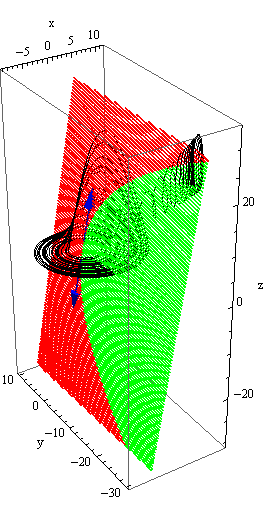
\includegraphics[width=0.16\textwidth]{robbins3-7a}
(b)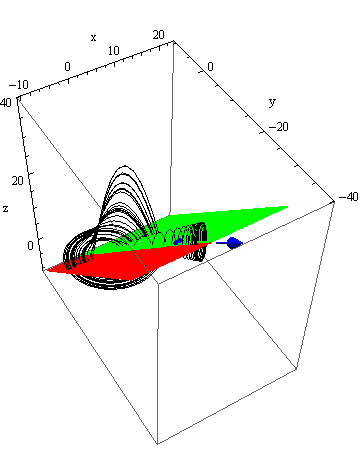
\includegraphics[width=0.24\textwidth]{robbins3-7b}
(c)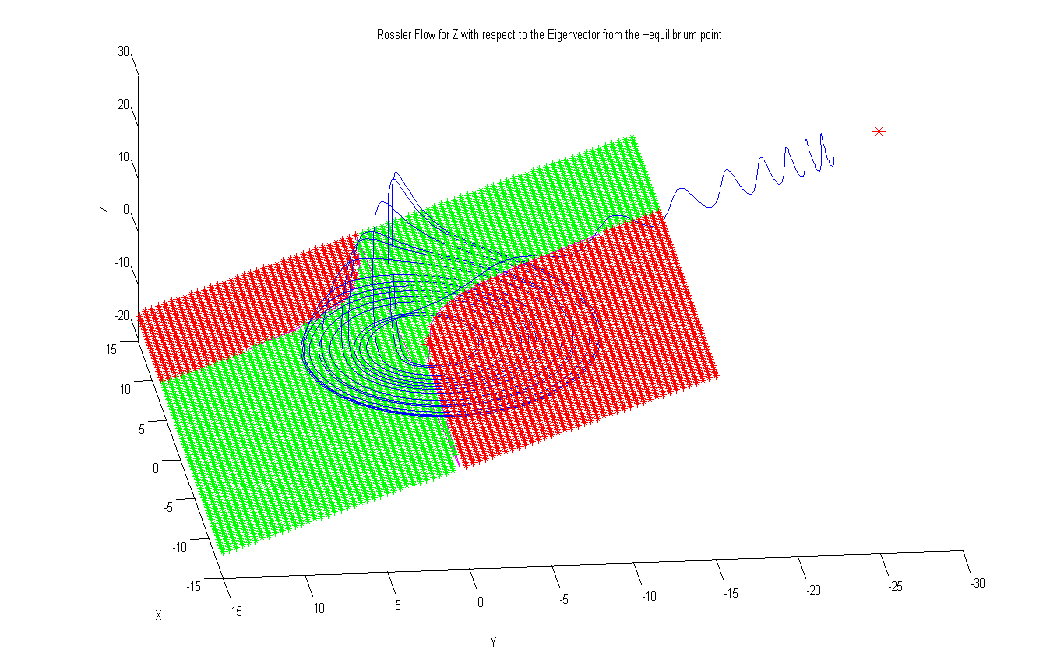
\includegraphics[width=0.44\textwidth]{wadsworth3-7a}
   \caption{\label{fig:robbins3-7}
    (a)
A section as in \refFig{fig:A29PoincBad}\,({\it b}), correctly centered
centered on $\ssp_{-}$ (Robbins).
    (b)
A section centered on $\ssp_{+}$ (Robbins).
    (c)
(Wadsworth).
}
\end{figure}
%%%%%%%%%%%%%%%%%%%%%%%%%%%%%%%%%%%%%%%%%%%%%%%%%%%%%%%%%%%%%%%%%%%%%

%%%%%%%%%%%%%%%%%%%%%%%%%%%%%%%%%%%%%%%%%%%%%%%%%%%%%%%%%%%%%%%%%%%%%
\begin{figure}
   \centering
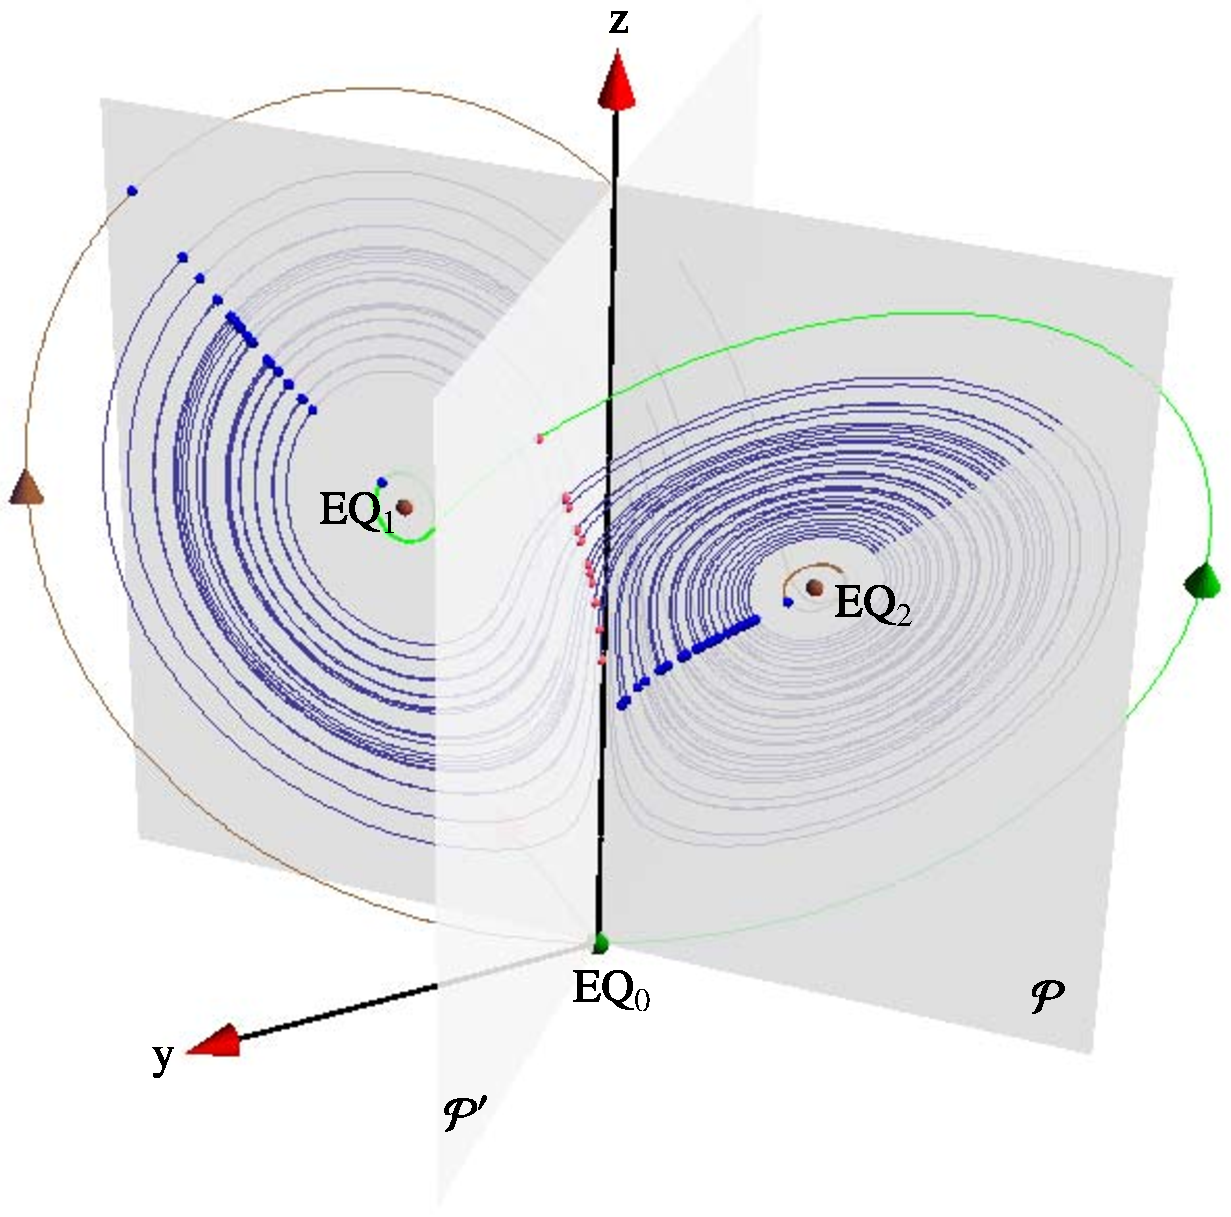
\includegraphics[width=0.40\textwidth, clip=true]{lorenz2Poinc}
   \caption{
Lorenz flow cut by  $y=x$ Poincar\'e section plane $\PoincS$ through the
$z$ axis and both $\EQV{1,2}$ \eqva. Points where flow pierces into
section % $\PoincS$ are marked by dots. To aid visualization of the flow
near the $\EQV{0}$ \eqv, the flow is cut by the second Poincar\'e
section,  $\PoincS'$, through $y=-x$ and the $z$ axis.
\hfill (from E. Siminos, ChaosBook.org)
%       \(\sigma = 10, b= 8/3, \rho = 28\,.\)
} \label{fig:LorenzSect}
\end{figure}
%%%%%%%%%%%%%%%%%%%%%%%%%%%%%%%%%%%%%%%%%%%%%%%%%%%%%%%%%%%%%%%%%%%%%


Along with continuous symmetries come important classes of invariant
solutions referred to as `relative' or `equivariant'
\rf{Huyg1673,Poinc1896}. One expects to find relative
equilibria and \rpo s\rf{Rand82}, associated with the translational
and rotational symmetries of the flow.


\subsection{R\"ossler unstable manifold curvilinear distance}

{\bf [2012-04-10 Predrag]} gave up on Keith's \reffig{fig:RoessRetMap}
and the yet undrawn {R\"ossler return map}.

%%%%%%%%%%%%%%%%%%%%%%%%%%%%%%%%%%%%%%%%%%%%%%%%%%%%%%%%%%%%%%%%%%%%%
\begin{figure}
\begin{center}
(a) % 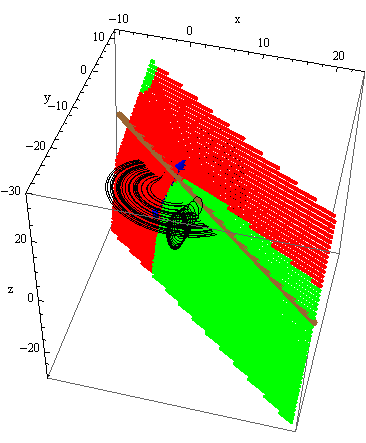
\includegraphics[width=0.30\textwidth,clip=true]{RoessSct1}
(b) 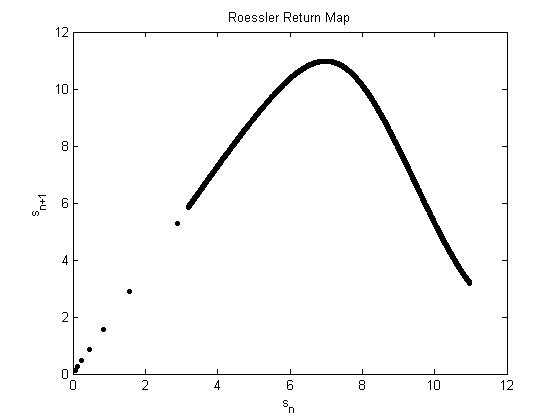
\includegraphics[width=0.30\textwidth,clip=true]{RoessRetMap}
\end{center}
  \caption{
(a) R\"ossler strange attractor section of \reffig{RoessSct1}
(b) R\"ossler return map for curvilinear distance as measured
along the unstable manifold section (the method of
\refref{Christiansen97}, see \refrefs{DasBuch,Basu07}).
  }
\label{fig:RoessRetMap}
\end{figure}
%%%%%%%%%%%%%%%%%%%%%%%%%%%%%%%%%%%%%%%%%%%%%%%%%%%%%%%%%%%%%%%%%%%%%



\subsection{Symmetries of flows}
\label{s:symmFL}

													\toCB
emphasize that our turbulent states are \emph{not} localized
three-dimensional solitary waves as quasi-particles -
\reffig{fig:A27-pipeSymms} might be misleading. Our solutions are global,
distributed over the whole volume.

Any state in the  group orbit set $\pS_{\ssp}$ is physically equivalent
to any other. The action of a symmetry group thus stratifies the
\statesp\ into a union of group orbits, \reffig{fig:BeThTraj}\,{(a)}.

While in the case of \SOn{2} symmetry a \reqv\ traces out a loop in the
full \statesp (see \reffig{fig:CLf01group}, e.g.), for a
higher-dimensional continuous symmetry it explores the group orbit
$\pS_{\REQV{}{}}$ quasi-periodically, so a \reqv\ is \emph{not} a \po.
Rather, as all states in this group orbit are physically the same state
for all time, this is a generalized \eqv\ state.

Continuous symmetry parameters (`phases' or `shifts')
$\{\gSpace_j\}=\{\phi_p,\shift_p\}$ are real numbers, ratios
$\pi/\gSpace_j$ are almost never rational, and \rpo s are almost never
eventually periodic; the time evolution of a relative periodic point thus
sweeps out quasi-periodically the $3$\dmn\ group orbit $\pS_p$ without
ever closing into a \po, unless the dynamics is restricted to a
discrete-symmetry invariant subspace (\reffig{fig:CLf01group}).

\subsection{Symmetry-induced coordinate frames}
\label{s:symmIndCoo}

At least locally, presence of a continuous symmetry suggests two
natural mutually orthogonal basis vectors, the group action tangent and
curvature vectors.

Consider the one-parameter rotation group \SOn{2} acting on a smooth
periodic function $u(\gSpace + 2\pi) = u(\gSpace)$ defined on domain
$\gSpace \in [0,2\pi)$, expanded in the Fourier basis
\refeq{eq:ksexp}.
    \PC{replace this by the original, 2\dmn\  real \SOn{2}  representation}
Parametrize the forward
translation by the continuous parameter $\phi$,
\(
    \LieEl(\phi)\,u(\gSpace) = u(\gSpace-\phi)
\,,
\)
or, in the Fourier basis,
\(
   \LieEl(\phi) \,\ssp = \mathrm{diag}\{ \mathrm{e}^{-\mathrm{i}m\phi} \} \,\ssp
\,.
\)
The tangent to the group orbit at the point $\ssp$ is then given by
the first derivative with respect to the group parameter,
\bea
   {\bf t}(\ssp) &=&
   \lim_{\gSpace\to 0}
   \left(\LieEl(\gSpace)\,\ssp - \ssp\right)/\gSpace
   = \mathrm{diag}\{ -\mathrm{i}m \} \, \ssp = \Lg \ssp,
\label{eq:tang}
\eea
where $\normVec$ is a unit vector normal to the tangent. The pair of unit vectors
    \PC{2011-10-28
    ``As $\Norm{\LieEl(\gSpace)\slicep}$ is a constant, for the group tangent
    vector $\Lg_\gSpace \slicep$ evaluated at $\slicep$ \refeq{eq:tang}
    %GroupTangField} is normal to $\slicep$, and the term
    $\braket{\slicep}{\Lg_\theta\,\slicep}$ vanishes ($\Lg_{\theta}$ is
    antisymmetric).''
The state vector $\ssp$ is not normal to \normVec(\ssp), as $\braket{\ssp
\Lg^2}{\ssp} = - \Norm{\groupTan(\ssp)}^2 \neq 0$, but can one use it to
produce from $\ssp$ the 3. local eigenbasis unit vector? Have not thought
that through. If we do that here, need to rewrite text leading to
\refeq{PCsectQ0}.
    }
\beq
\{{\be_n},{\be_{n+1}}\} =
\{\groupTan(\ssp)/\Norm{\groupTan(\ssp)},\normVec(\ssp)\}
\ee{FrenetFrame}
forms a local orthogonal Frenet-Serret frame at $\ssp$, and can be useful
in constructing the \statesp\ basis vector set \refeq{intrSspTraj}.

\begin{figure}
  \centering
(a)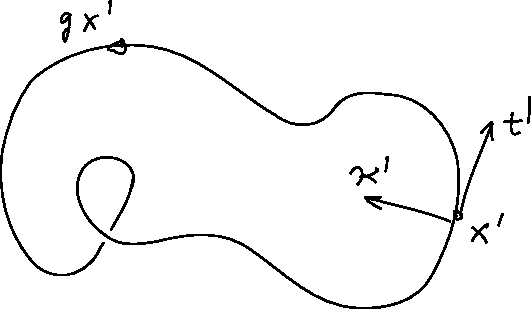
\includegraphics[width=0.20\textwidth]{A29FSframe}
(b)%\includegraphics[width=0.45\textwidth]{2840GOt135th0}
  \caption{\label{fig:2840GOt135th0}
    %\label{fig:M1groupOrb}
Projections of group orbits of two states $\ssp$ (in $\approx
100,000$-dimensional {\statesp}) onto a stationary Frenet-Serret frame
given by unit vectors in the directions
$\{\groupTan_z(\ssp'),\groupTan_\theta(\ssp'),\normVec_z(\ssp')\}$ (see
\refeq{FrenetFrame}). The group orbit is generated by
$\LieEl(0,\shift)\,\ssp$, i.e. by axial shifts, and plotted relative to the
point $\ssp'$.
In  (b) $\ssp$ is a strongly nonlinear chaotic state.
Group orbits are only topologically circles, and inflections are possible
when $\ssp$ is not so close to $\ssp'$.
%{APW 111027 For N2_UB, only see mild distortions;
% see fig 15(b) of dailyBlog}
  }
\end{figure}

For a time-dependent group parameter
$\gSpace$, the phase speed $\dot{\gSpace}$ along the group tangent
evaluated at the \statesp\ point $\ssp$ (the `Cartan derivative') is
given by
\beq
\LieEl^{-1}\dot{\LieEl} \,\ssp % =e^{-\gSpace \cdot \Lg} \,
     =\mathrm{e}^{-\gSpace \Lg} \,
\left(\frac{\mathrm{d} ~~}{\mathrm{d} \, \zeit} \, % e^{\gSpace \cdot \Lg}\ssp
                             \mathrm{e}^{\gSpace \Lg}\right)\ssp
    =\dot{\gSpace} \, \groupTan(\ssp)
%    =\dot{\gSpace}\cdot \groupTan(\ssp)
\,.
\ee{CartanDer}



\subsubsection{Ring of Fire}

%%%%%%%%%%%%%%%%%%%%%%%%%%%%%%%%%%%%%%%%%%%%%%%%%%%%%%%%%%%%%%%%%%%%%
\begin{figure}
(a) 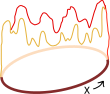
\includegraphics[width=0.145\textwidth]{A27RoFire}
(b) 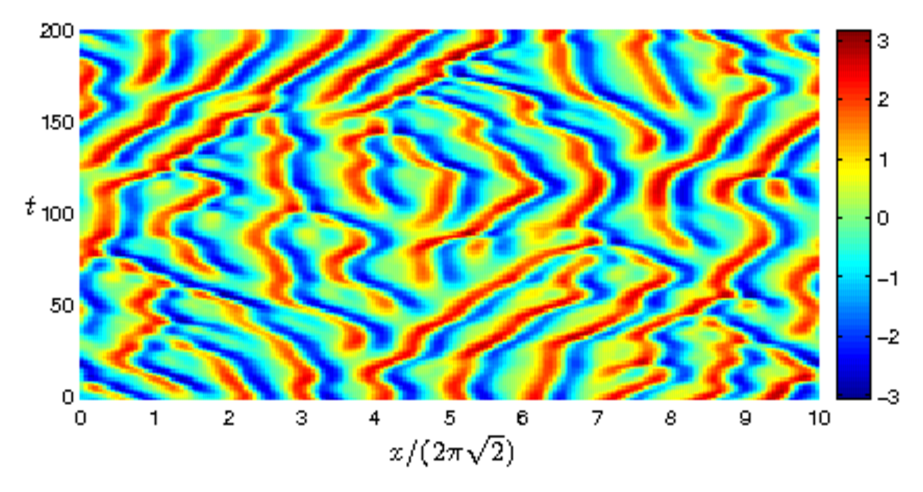
\includegraphics[width=0.255\textwidth]{ks_largeL_cbar_200}
  \caption{
The Ring of Fire, visualized as
    (a)
a Bunsen burner flame flutter, with $u=u(x,t)$ the velocity of the
flame front at position $x$ and time $t$;
    (b)
a spatiotemporal plot (from \wwwcb{}). The symmetry of the system is
$\On{2}$; a rotation of a solution is also a solution.
  }
\label{fig:A27RoFir}
\end{figure}
%%%%%%%%%%%%%%%%%%%%%%%%%%%%%%%%%%%%%%%%%%%%%%%%%%%%%%%%%%%%%%%%%%%%%

Bunsen burner, invented by G\"ottingen chemistry prodigy Robert Bunsen in
1855, entered popular culture in  in 1963 as Johnny Cash
\etal\rf{CaCaKi63} ``\HREF{http://www.youtube.com/watch?v=mIBTg7q9oNc}
{Ring of Fire}'' (\reffig{fig:A27RoFir}), and its flame front
instabilities were modeled in 1976 by Kuramoto\rf{ku} and
Sivashinsky\rf{siv} by one of the simplest nonlinear PDEs that exhibit
spatiotemporally chaotic behavior. The time evolution of the  flame front
velocity $u=u(x,t)$ on a periodic domain $u(x,t) = u(x+L,t)$ is given by
\beq
  u_t = F(u) = -u\,u_x-u_{xx}-u_{xxxx}
    \,.
\ee{ks}
Spatial periodicity $u(x,t)=u(x+L,t)$
makes it convenient to work in the Fourier space,
\beq
  u(x,t)=\sum_{k=-\infty}^{+\infty} a_k (t)\, e^{ i k x /\tildeL }
\,,
\ee{eq:ksexp}
with the $1$-dimensional PDE \refeq{ks}
replaced by an infinite set of
ODEs for the complex Fourier coefficients $a_k(\zeit)$:
\beq
\dot{a}_k= \pVeloc_k(a)
     = ( q_k^2 - q_k^4 )\, a_k
    - i \frac{q_k}{2} \sum_{m=-\infty}^{+\infty} a_m a_{k-m}
\,,
\ee{expan}
where $q_k = 2\pi k/L$.


\subsection{Symmetries of pipe flow}
\label{s:SymmPipe}
% former siminos/atlas/symm.tex

In the literature
(see, \eg\ \cite{Recke2010}) such \SOn{2} is often referred to as the
circle group $S^1$, also denoted `one-torus' $T^1$.

\section{How to slice}
\label{s:algorithm}

This problem is here resolved by the
{\mslices}, in which
the group orbit of any full-flow structure is represented by a single
point (see \reffig{fig:BeThTraj}), the group orbit's intersection with a
fixed hypersurface, or the \emph{`\slice'}.

Our guiding principle is to chose a \slice\ such that the distance
between a `{\template}' state {\slicep} and nearby group orbits is
\emph{minimized}, \ie, identify the point $\sspRed$ on the group orbit
\refeq{sspOrbit} of a nearby state $\ssp$ which is the closest match to
the {\template} point {\slicep}.

\refFig{fig:sliceimage}, new proposal: take points on the good,
    blue \po, run each along the group orbit until $\sspRSing \in S$
    where it intersects the \sliceBord, see \refeq{sspRSing}, and thus plot
    the border of where the local slice ends, once on the left, and once
    on the right of the {\template}. Catch - I have not thought this
    through, not sure that the condition \refeq{sspRSing} can be
    satisfied on every group orbit...

We have seen that in presence of the continuous $\SOn{2}$ symmetry
\reqva\ and \rpo s are 2- and 3-dimensional manifolds of physically
equivalent states. How are we to compare a pair of such states? We shall
do this here by determining the minimal distance between them.

In particular, even though the
simplest solutions (laminar, \etc) often capture important physical
features of a flow, most \eqva\ and short \po s have nontrivial
symmetries and thus are not suited as choices of symmetry-reducing
{\template s}.

%%%%%%%%%%%%%%%%%%%%%%%%%%%%%%%%%%%%%%%%%%%%%%%%%%%%%%%%%%%%%%%%%%%%%
\begin{figure}
   \centering
(b)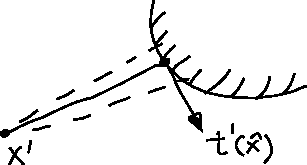
\includegraphics[width=0.20\textwidth]{A28extremum}
   \caption{\label{fig:A28extremum1}
    (b) Extremal condition \refeq{PCsectQ0}, replaced by
    \reffig{fig:A28extremum}
}
\end{figure}
%%%%%%%%%%%%%%%%%%%%%%%%%%%%%%%%%%%%%%%%%%%%%%%%%%%%%%%%%%%%%%%%%%%%%

In particular, if  \sspRed\ is a point on a \reqv, % \refeq{phaseVel},
the full \statesp\ velocity equals the {\phaseVel}, and $\velRed(\sspRed)
= 0$, \ie, \reqva\ are always reduced to \eqva\ in the \reducedsp.


\subsection{Rotation into the \slice}

As long as the norm is discretization independent, the \slice\ condition
\refeq{PCsectQ0} is independent of the numerical representation $\ssp$ of
the flow $\vec{u}$, be it finite difference, spectral, and so on. The
slice condition is solved for $\shift$ every few time steps using
Newton's method, where a good initial guess for $\shift(\zeit)$ is
obtained from the previous value and $\dot{\shift}(\zeit)$.

To avoid this, a global
atlas has to be pieced together from local \slice\ charts, fixed by
a well-chosen set of
\template s $\slicep{}^{(j)}$.
Shifts $\shift_j(\zeit)$ are tracked for each local \slice\ chart $\pS{}^{(j)}$,
such that the next $\shift_{j+1}(\zeit)$ is selected at intersection with
$\pS{}^{(j+1)}$
to minimize $\Norm{{\ssp}-{\ssp_i}}$.

%\APW{111104 The first sentence requires simplifying!}
As group orbits % of compact Lie groups
are smooth manifolds, have natural linear
representations (under linear action of a symmetry group, \statesp\
decomposes into a sum over irreducible subspaces), and have natural local
coordinate frames (the group tangent, curvature Frenet-Serret frames
\refeq{FrenetFrame}), good \slice s should be easier to construct than
the elusive ``good'' Poincar\'e sections of the time-evolution flows.
Indeed, as a generic \slice\ \refeq{PCsectQ0} is the set of all
group-orbit points closest to a given {\template}, it slices the group
orbits of \emph{all} full \statesp\ points\rf{FrCv11}. However, for a
nonlinear flow, there is no single \slice\ that really does the job: our
\slice\ is locally a hyperplane, expected to be a good description of
solutions similar to a given {\template} in some open neighborhood. The
variational distance condition \refeq{PCsectQ0} is only an extremum
condition, and as the group orbits of highly nonlinear states are highly
contorted (see \reffig{fig:2830GO6}\,{\it b}), they can have many
extrema, and multiple sections by a \slice\ hyperplane. For example, an
\rpo\  torus is always intersected by a \slice\ hyperplane in two or more
sections, see \reffig{fig:sliceimage}.

A single
\slice\ hyperplane cannot do the job well. As the {\nws} of the dynamics is a
highly contorted, nonlinear curved manifold embedded in a
high-dimensional \statesp, any such linearization is good only locally: a
single {\template} cannot be a good match  globally.


    \ifdraft\color{blue}
        {\bf 2012-03-15 Predrag} \refFig{fig:sliceimage}, new proposal:
        take points on the good, blue \po, run each along the group orbit
        until $\sspRSing \in S$ where it intersects the \chartBord, see
        \refeq{sspRSing}, and thus plot the border of where the local
        slice ends, once on the left, and once on the right of the
        {\template}. Catch - I have not thought this through, not sure
        that the condition \refeq{sspRSing} can be satisfied on every
        group orbit...
    \color{black}\fi

It should be emphasized that we never need to integrate the reduced
equations \refeq{EqMotMFrame}; numerical simulations are always carried
out in the full \statesp. Slicing is implemented as postprocessing of
numerical or experimental data, by rotating full \statesp\ trajectories
into the \slice, as in \reffig{fig:sliceimage}.

The apparent divergence in {\phaseVel} \refeq{reconstrEq} is a
non-physical artifact of the symmetry reduction by tangent hyperplanes,
but a numerical nuisance nevertheless. Here is how we avoid it.

Thus, in order to chart the \statesp\ of a chaotic flow, a set
of local \slice\ hyperplanes is needed to capture all of the asymptotic
dynamics. The choice of local \slice s should reflect the dynamically
dominant patterns seen in the solutions of nonlinear PDEs.

``The origin'' or the invariant, fixed-point subspace is a
high-dimensional center space of points not moved by $\Lg_{\theta}$. For
\pCf\ it is the space plumbers prefer to compute in, even though all
turbulence is in the full \statesp. The reason why I really, really want
us to understand what is going on with our atlas in \reffig{fig:A29-2slices}
is that the singularities might be genuine, due to close passages to this
center space, and not taken care of by $\sspRSing$ (which all also
include the `origin'), not just due to bad choice of \template s.

In general, these polynomials are non-unique and $m \geq d$, so
that the flow becomes embedded in a larger m-dimensional state space.
While these polynomials are linearly independent, they are functionally
dependent by a set of relations called syzygies. The syzygies constrain
the flow to lower dimensional, but non-trivial, manifolds in the
m-dimensional space.

Sometimes the determination of a Hilbert basis can be informed by
intuition about nonlinear preserved quantities such as rotationally
invariant length $r^2 = x_1^2 + x_2^2 + ... + x_d^2$. In general,
however, there is no general strategy for creating a useful Hilbert
basis.

\subsection{Physical dimension: covariant Lyapunov vectors}

\subsection{Dynamically important solutions and Newton's method}
\label{s:reqva}

Without symmetry reduction, the detection of the nearest recurrence of a
state near a previous state, earlier on the the same trajectory, would
require the calculating the minimum over all possible shifts. Within the
symmetry-\reducedsp\ the determination of recurrences is simple, as the
slices are constructed by requiring that the slice points are the minimum
distance points between the group orbits of the two states.

These are not the `modes' of the fluid; {they
do not provide a decomposition of the flow into a sum of components at
different wavelengths, or a basis for low-dimensional
modeling.} Each such solution spans the whole range of physical scales of
the turbulent fluid, from the outer wall-to-wall scale, down to the
viscous dissipation scale. Numerical computations require sufficient
resolution to cover all of these scales, so no {global} dimension
reduction is likely.

        {\bf PC 2011-10-18} Note also that the rotation of a fluid flow
        into a \slice\ {\em is not} an average over the 3D pipe azimuthal
        angle, it is the full snapshot of the flow embedded in the
        $\infty$-dimensional \statesp.

As a generic \slice\ \refeq{PCsectQ0} is the set of all group-orbit
points closest to a given {\template}, it slices the group orbits of
\emph{all} full \statesp\ points\rf{FrCv11}.

The role of invariant solutions is
to partition the $\infty$-dimensional \statesp\ into a finite set of
neighborhoods visited by a typical long-time turbulent fluid state.

Ignore it at
your own peril; the invariant solutions found by restricting
searches to the discrete-symmetry invariant subspaces have little if
anything to do with the full \statesp\ explored by turbulence, not more
than the \eqv\ points of the Lorenz equation have to do with its strange
attractor.

 As the symmetries do not act on
the invariant subspaces, for them $\sliceTan{} = 0$, and they are
contained within all slices.
